\documentclass[12pt]{exam}
%\documentclass[12pt]{article}
\usepackage[letterpaper, margin=0.75in]{geometry}
\usepackage{graphicx}
\usepackage{enumitem}
\usepackage{booktabs}
\usepackage{amsmath}
\usepackage{tabularx}
\usepackage{color}
\usepackage{textcomp}

\begin{document}
\footer{}{Page \thepage\ of \numpages}{}

\begin{flushright}
\makebox[0.5\textwidth]{\large Name:\enspace\hrulefill}
\vspace{0.2in}

\makebox[0.5\textwidth]{\large Date:\enspace\hrulefill}
\end{flushright}

\begin{center}

\includegraphics[width=10cm]{../images/logo.png}
\end{center}

\begin{center}
\noindent{\LARGE Conceptual Physics \\ Class 6 Questions \\ March 16, 2018 \\}
\end{center}
\vspace{0.2in}

\clearpage
\begin{questions}
\question When an object moves, the force of friction does work on it. Where does this energy go?
\vspace{1.5in}

\question Can kinetic energy ever be less than zero? Why or why not? (From \textit{Light and Matter}, Chapter 11 Question 2)
\vspace{1.5in}

\question Two balls are released from a certain height. One is dropped straight down, the other rolls down an incline.
\begin{center}
	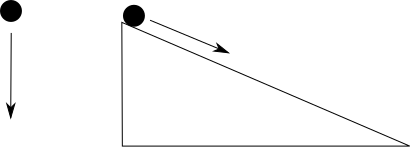
\includegraphics[width=2in]{../images/droppingBalls.png}
\end{center}
\begin{parts}
	\part Assuming no friction, which one has the greatest speed when it reaches the ground?
	\vspace{0.5in}
	\part Assuming no friction, which one reaches the ground first?
	\vspace{0.5in}
	\part Assuming there is friction, which one has the greatest speed when it reaches the ground?
	\vspace{0.5in}
\end{parts}

\question You throw a steel ball up in the air. How can you prove based on the conservation of energy that it has the same speed when in falls back into your hand? What if you throw up a feather - is energy not conserved in that case? (From \textit{Light and Matter}, Chapter 12 Discussion Question A)
\vspace{1.5in}

\question Anya and Ivan lean over a balcony side by side. Anya throws a penny downward with an initial speed of 2 m/s. Ivan throws a penny upward with the same speed. Both pennies end up on the ground below. Compare their kinetic energies and velocities on impact (as in, which is bigger, smaller, pointing up/pointing down, etc.)
\vspace{2in}


\question If you hold a 2~kg object at a steady height of 1.5~m, and walk forward at a constant speed of 5~m/s for 2~seconds, how much work do you do on the object?
\vspace{2in}

\question Hydroelectric power (water flowing over a dam to spin turbines) appears to be completely free. Does this violate conservation of energy? If not, what is the ultimate source of the electrical energy produced by a hydroelectric plant? (From \textit{Light and Matter}, Chapter 11 discussion question A)
\vspace{3in}

\clearpage

\question Two runners, each of mass $m$, are running with speed $v$ in opposite directions. What is their total kinetic energy?
\begin{center}
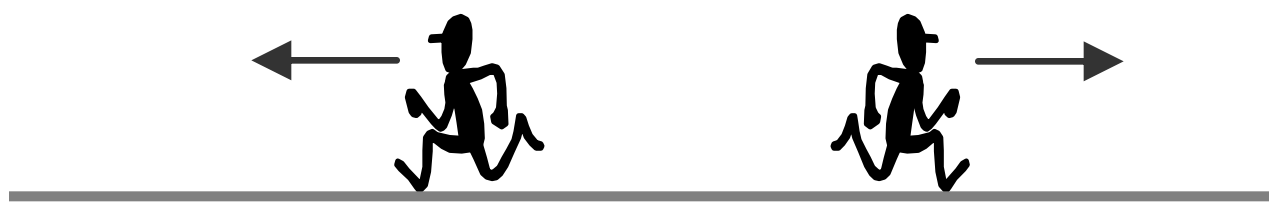
\includegraphics[width=3in]{../images/runnersOpposite.png}
\end{center}
	\begin{parts}
		\part 0 
		\part $\frac{1}{2}mv^2$
		\part $m v^2$
		\part $2 m v^2$
	\end{parts}
	
\question The two runners, each of mass $m$, are running are now running in the same direction with speed $v$. What is their total kinetic energy now?
\begin{center}

\includegraphics[width=3in]{../images/runnersSame.png}
\end{center}
	\begin{parts}
		\part 0 
		\part $\frac{1}{2}mv^2$
		\part $m v^2$
		\part $2 m v^2$
	\end{parts}

\question Consider 3 moving cars:
	\begin{enumerate}
		\item Car 1 moves at a constant speed and in a constant direction.
		\item Car 2 moves at a constant speed but \textit{changes} direction.
		\item Car 3 moves in a constant direction but changes its \textit{speed}.
	\end{enumerate}
Which of the following cars has (have) constant kinetic energy?
\begin{parts}
	\part Car 1
	\part Car 1 and Car 2
	\part Car 2 and Car 3
	\part Car 1 and Car 3
	\part Car 1, Car 2, and Car 3
	\part None of the above: they all have changing kinetic energy
\end{parts}
\vspace{0.3in}
\clearpage
\question
Consider the following point charges, with equal and opposite electrical charge, being held apart at distances $r$ and $2r$.
\begin{center}
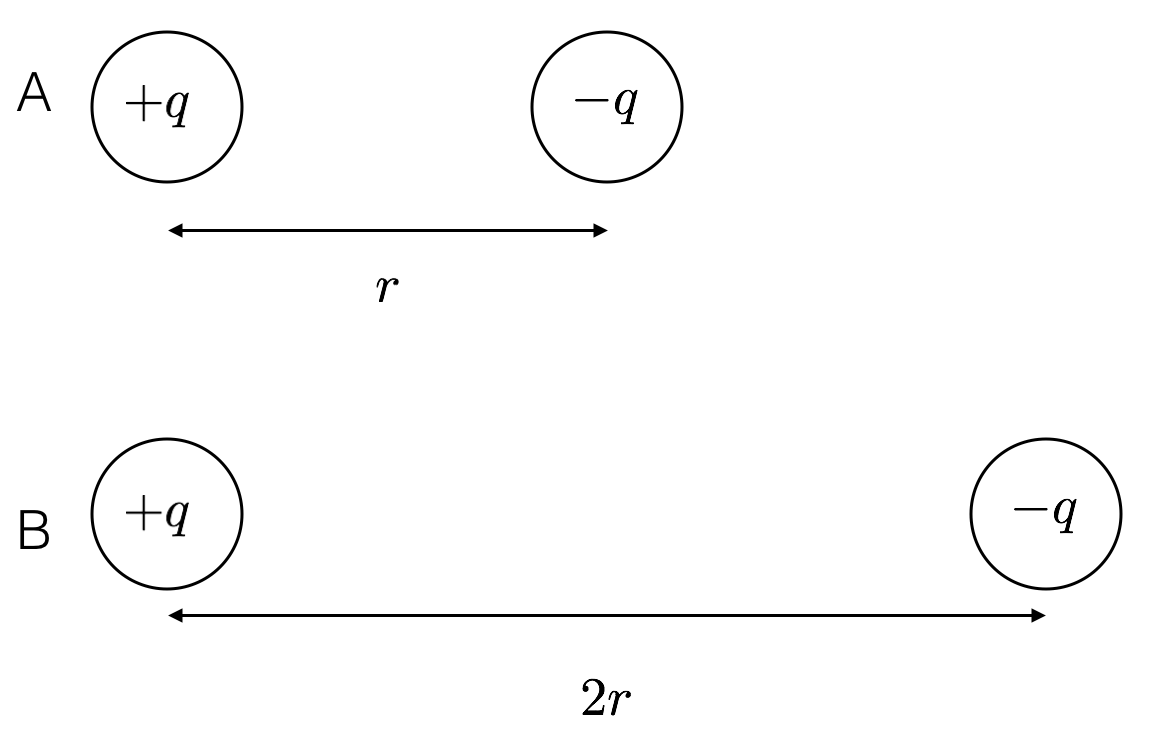
\includegraphics[width=0.5\textwidth]{../images/coop9_chargeopp.png}
\end{center}
\begin{parts}
\part In which configuration, A or B, do the charges feel a greater magnitude of electrical force (\textit{i.e.}, more attracted or more repelled)?
\vspace{0.5in}
\part In which configuration, A or B, do the charges have a greater potential energy?
\vspace{0.5in}
\end{parts}

\question Now consider the following point charges, with equal electrical charge of the same sign, being held apart at distances $r$ and $2r$.
\begin{center}
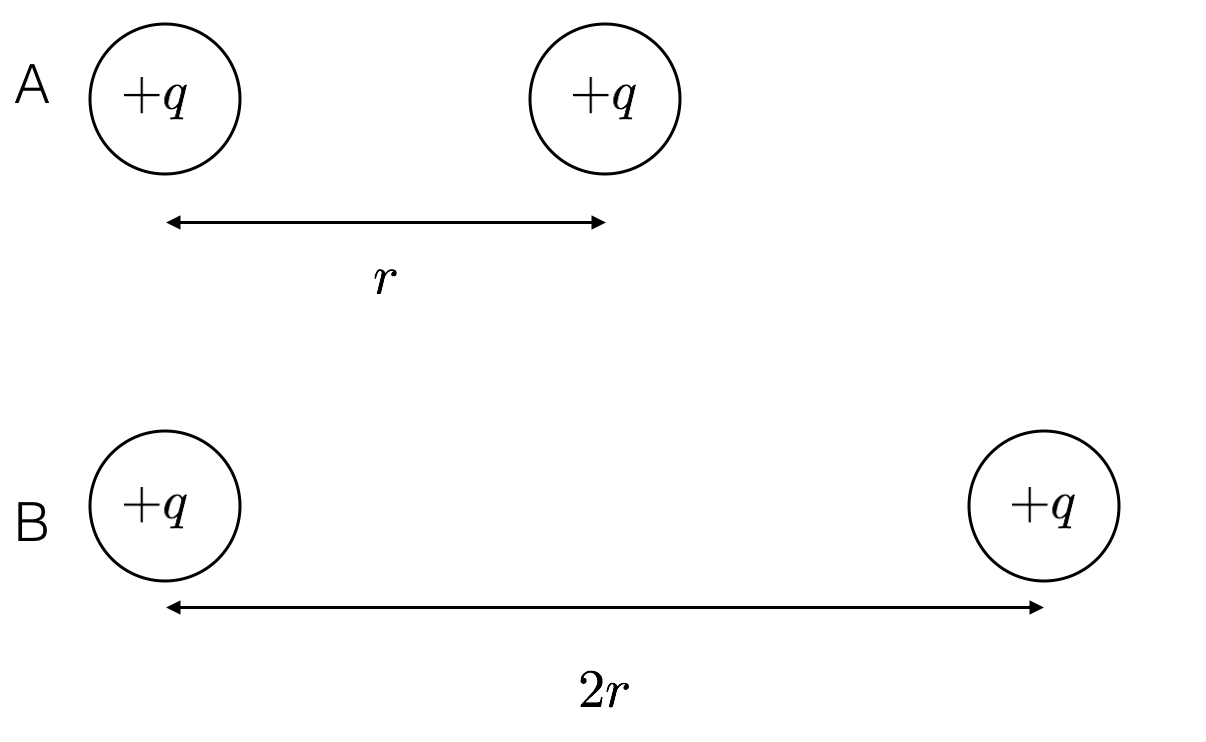
\includegraphics[width=0.5\textwidth]{../images/coop9_chargesame.png}
\end{center}
\begin{parts}
\part In which configuration, A or B, do the charges feel a greater magnitude of electrical force (\textit{i.e.}, more attracted or more repelled)?
\vspace{0.5in}
\part In which configuration, A or B, do the charges have a greater potential energy?
\vspace{0.5in}
\end{parts}

\question At a location in space far from any other objects, two moving asteroids (asteroid I and asteroid II) pass each other. Diagram 1 shows the two asteroids at one point in time, and diagram 2 shows them some time later.
\begin{center}
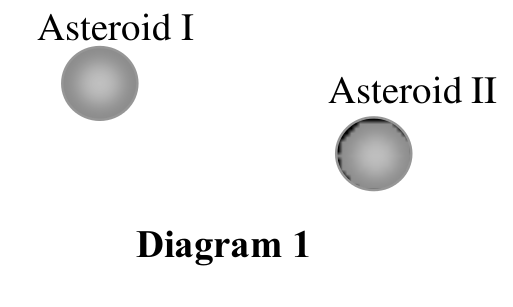
\includegraphics[scale=0.25]{../images/asteroids1.png} \hspace{0.5in} 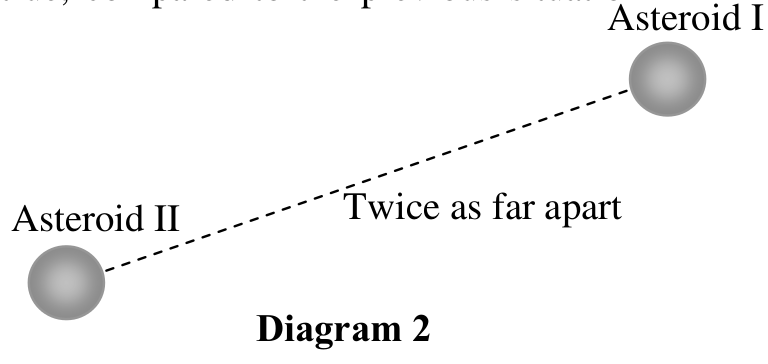
\includegraphics[scale=0.25]{../images/asteroids2.png}
\end{center}
Which of the following statements are correct?
\begin{parts}
	\part The potential energy increased, the kinetic energy increased
	\part The potential energy increased, the kinetic energy decreased
	\part The potential energy increased, the kinetic energy remained constant
	\part The potential energy decreased, the kinetic energy increased
	\part The potential energy decreased, the kinetic energy decreased
	\part The potential energy decreased, the kinetic energy remained constant
	\part Energy is conserved, therefore both the kinetic and potential energy remained constant
\end{parts}
\clearpage

\question BONUS QUESTION: The following figure plots kinetic energy K and potential energy U of a two-particle system versus the distance $r$ between the two particles. From these curves we can conclude that the interaction between the two particles is:
\begin{center}

\includegraphics[width=3in]{../images/twoParticlesForce.png}

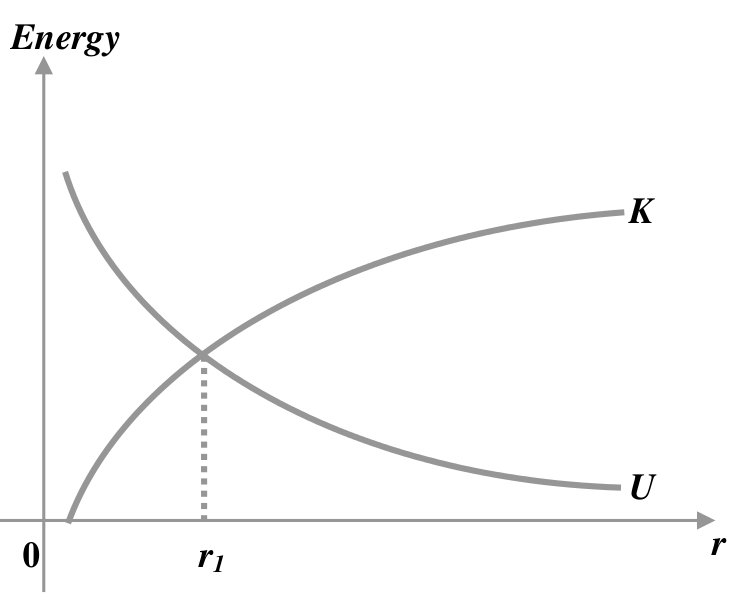
\includegraphics[width=3in]{../images/energyDistanceGraph.png}
\end{center}
\begin{parts}
	\part Repulsion
	\part Attraction
	\part Repulsion when $r < r_1$ and attraction when $r > r_1$
	\part Attraction when $r < r_1$ and repulsion when $r > r_1$
	\part Not enough information to determine
\end{parts}

\end{questions}

\end{document}
